\documentclass[12pt]{article}

\usepackage{lmodern}
\usepackage[T1]{fontenc}
\usepackage[utf8]{inputenc}
\usepackage[spanish, activeacute]{babel}
\usepackage{listings}
\usepackage{enumitem}
\usepackage{graphicx}
\usepackage{float}
\usepackage[hidelinks]{hyperref}
\usepackage{xcolor}

\definecolor{mygreen}{rgb}{0,0.6,0}
\definecolor{mygray}{rgb}{0.8,0.8,0.8}
\definecolor{mymauve}{rgb}{0.58,0,0.82}

\lstset{
backgroundcolor=\color{mygray},   
basicstyle=\ttfamily,        
breakatwhitespace=false,         
captionpos=b,                    
commentstyle=\color{mygreen},    
deletekeywords={...},            
escapeinside={\%*}{*)},          
extendedchars=true,              
keepspaces=true,                 
keywordstyle=\color{blue},       
language=Octave,                 
morekeywords={*,...},            
numbers=left,                    
numbersep=5pt,                   
numberstyle=iny\color{black}, 
showspaces=false,                
showstringspaces=false,          
showtabs=false,                  
stepnumber=1,                    
stringstyle=\color{mymauve},     
tabsize=2,                       
}

\graphicspath {{ assets/images/ }}

\title{Práctica 05 - Aplicación del clima}
\author{ 
    Wilson Aguilar \\
    \textsc{Plataformas Web} 
}

\begin{document}

\maketitle

\section{Inicio del proyecto y dependencias}

Esta aplicación se centra en el consumo de un servicio de internet y poder mostrar esos datos dentro de la aplicación.

En específico vamos a crear una aplicación que nos dara información del clima de alguna ciudad del mundo. Para ello nos vamos a conectar a una API que nos brinde esta información.

Para inicializar el proyecto ejecutamos el comando:
\lstinline{npm init -y}

Además, instalaremos las siguientes dependencias:

\begin{description}
    \item[Yargs] Nos ayudara con la creación de una app en consola.
    \item [Axios] Nos permite realizar peticiones http.
\end{description}

Para ello ejecutamos \lstinline{npm install --save yargs axios}

\begin{figure}[H]
    \centering
    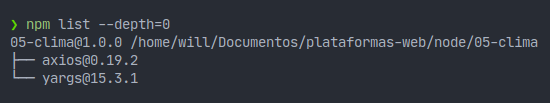
\includegraphics[scale=.8]{assets/images/dependences.png}
    \caption{Listado de dependencias del proyecto}
    \label{}
\end{figure}

\section{Configuración de yargs}

Yargs es un paquete de node que nos ayuda a crear aplicaciones de consola de una manera mucho mas sencilla. En este caso nuestra aplicación contara de 2 opciones, una para ingresar la ciudad de donde vamos a consultar la información del clima y la otra para solicitar información extra (humedad y presion).

\begin{figure}[H]
    \centering
    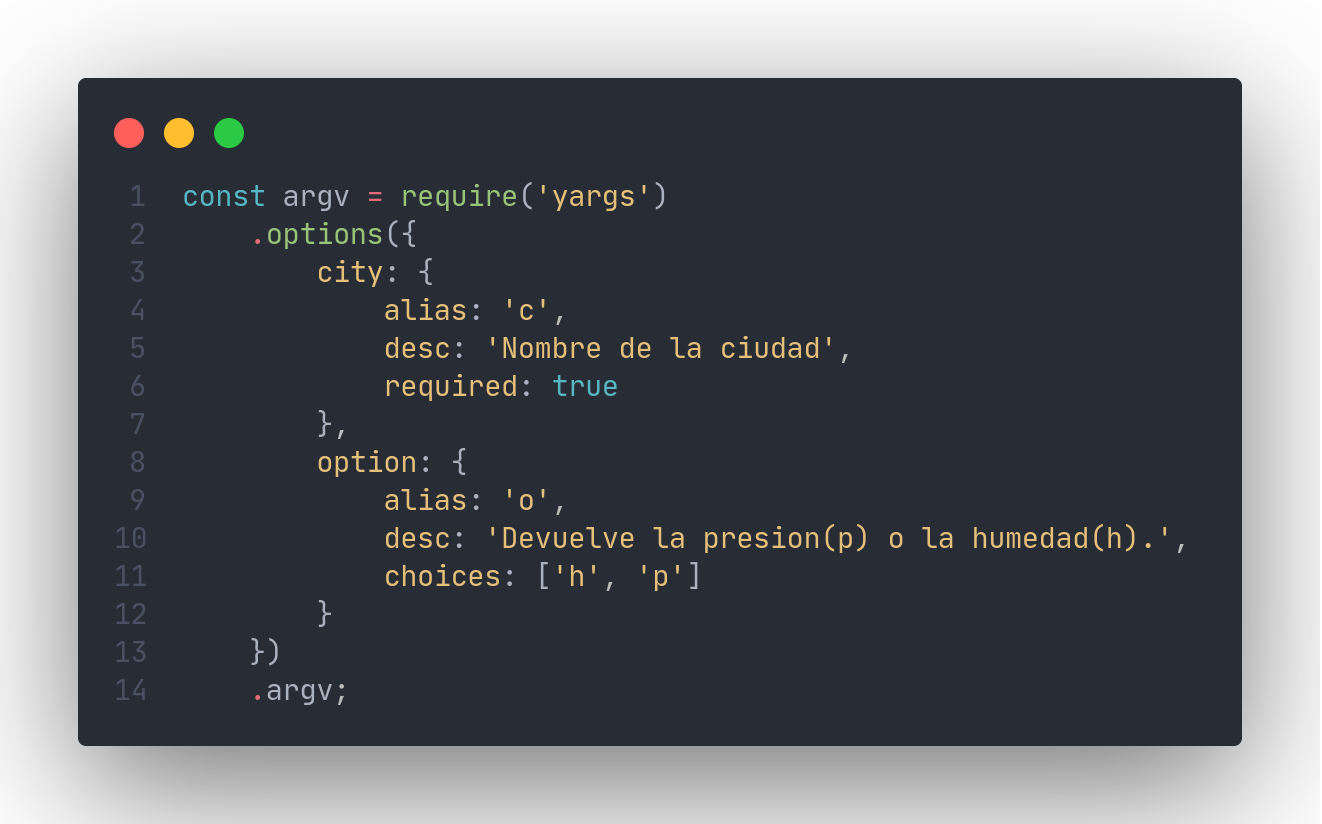
\includegraphics[scale=.25]{assets/images/yargs.png}
    \caption{Configuración del módulo yargs.}
\end{figure}

\section{Consumo de servicios}

\subsection{Open Weather Map}

Open Weather Map es un servicio en linea que nos proporciona datos méteorologicos. Nos conectaremos a esta API para recopilar la información que necesitamos. Para ello necesitamos crearnos una cuenta en este sitio para que nos proporcionen un token de acceso para poder solicitar datos al sitio.

\begin{figure}[H]
    \centering
    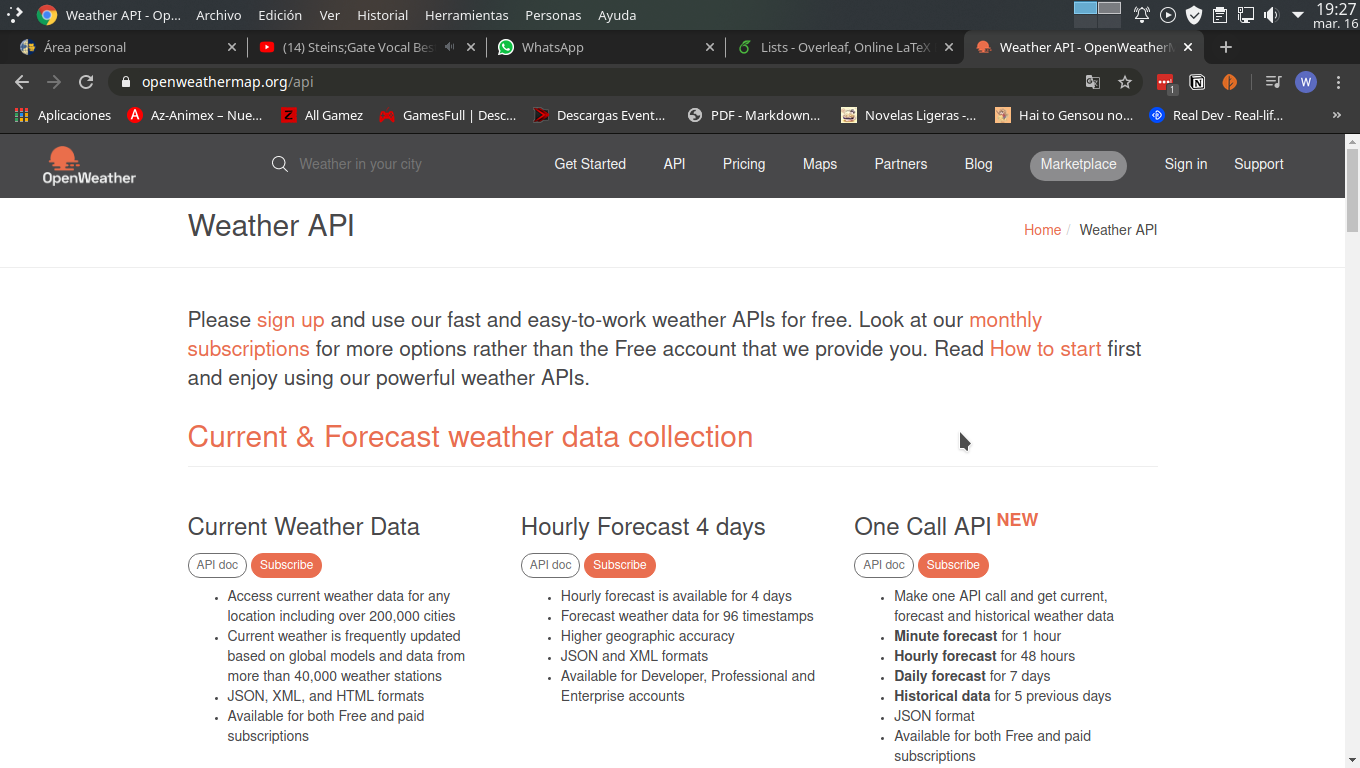
\includegraphics[scale=.35]{assets/images/api.png}
    \caption{Sitio oficial de Open Weather Map.}
\end{figure}

Dentro de la documentación de Open Weather Map podemos observar como podemos realizar una petición de los datos que solicitamos.

\begin{figure}[H]
    \centering
    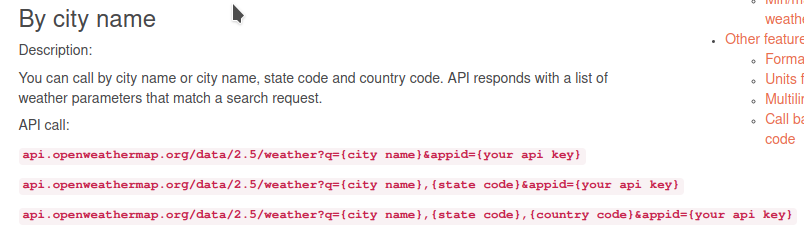
\includegraphics[scale=.5]{assets/images/api-2.png}
    \caption{Ejemplo de petición.}
\end{figure}

En este caso usaremos el enlace que nos proporciona la documentación para poder realizar pruebas y observar que datos nos devuelve.

El enlace que usaremos es el siguiente:

\url{api.openweathermap.org/data/2.5/weather?q={city}&appid={key}}

\begin{description}
    \item[city] Es el nombre de la ciudad que vamos a consultar.
    \item[key] Es el token que nos da la api para poder realizar peticiones.
\end{description}

\newpage

\subsection{Solicitar datos}

Para poder pedir los datos del clima que necesitamos debemos realizar una peticion http de tipo GET hacia la url mostrada anteriormente. Los navegadores web por defecto cuando ingresan a un sitio realizar esta peticion hacia el servidor solicitando la página, asi que usaremos este método para que pedir la información por medio del navegador.

\begin{figure}[H]
    \centering
    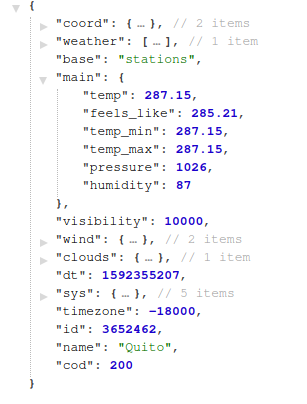
\includegraphics{assets/images/browser.png}
    \caption{Solicitando datos desde el navegador}
\end{figure}

Como observamos pedimos información acerca del clima de quito y nos devolvió estos datos en un formato json. Cuando hacemos peticiones hacia una API, por lo general nos dan una respuesta en este formato.

Tambien tenemos herramientas especializadas en realizar péticiones. Postman es una de ellas y muy famosa entre los desarrolladores. Postman no solo nos deja realizar péticiones GET, sino que todo tipo de péticiones, POST, PUT, OPTION, etc. Además de que nos deja modificar varios aspectos de estas, es un programa especializado para probar API's y realizar peticiones.

Ahora para realizar una peticion desde Postman solo debemos escoger el método a usar, en este caso GET, ingresamos la dirección y los parametros que son la q (query) y appid(key de api), esta vez añadimos un parametro mas que es metric y nos ayudara a que la temperatura que nos devuelve la API sea en grados celcious.

\begin{figure}[H]
    \centering
    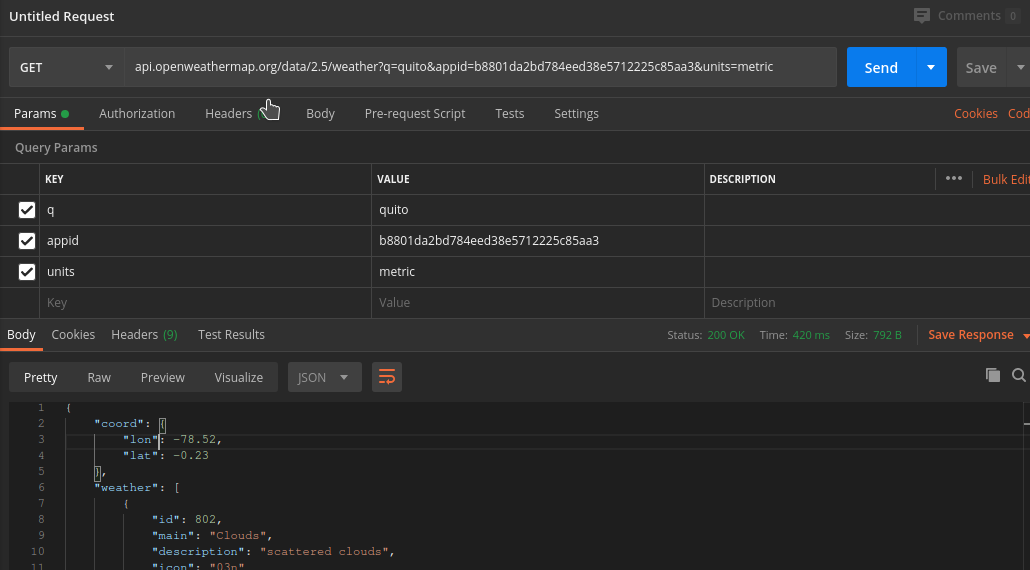
\includegraphics[scale=.5]{assets/images/postman.png}
    \caption{Peticion desde Postman}
\end{figure}

Como podemos observar postman es un poco mas complejo pero a cambio nos da mucha mas información acerca de como se realizo la peticion, vemos que la peticion fue exitosa con código de estado 200 ok y nos devolvio la misma información que el navegador.

\newpage

\section{Axios}

Para poder realizar peticiones http desde algun lenguaje de programación nos apoyamos de librerias que nos permitan realizar esta acción. Para Nodejs y javascript Axios es una buena opción, es sencilla de utilizar y tiene buen soporte de la comunidad.

\subsection{Configurando Axios}

Para tener nuestro código mejor ordenado separamos la configuración de axios en un archivo aparte.

\begin{figure}[H]
    \centering
    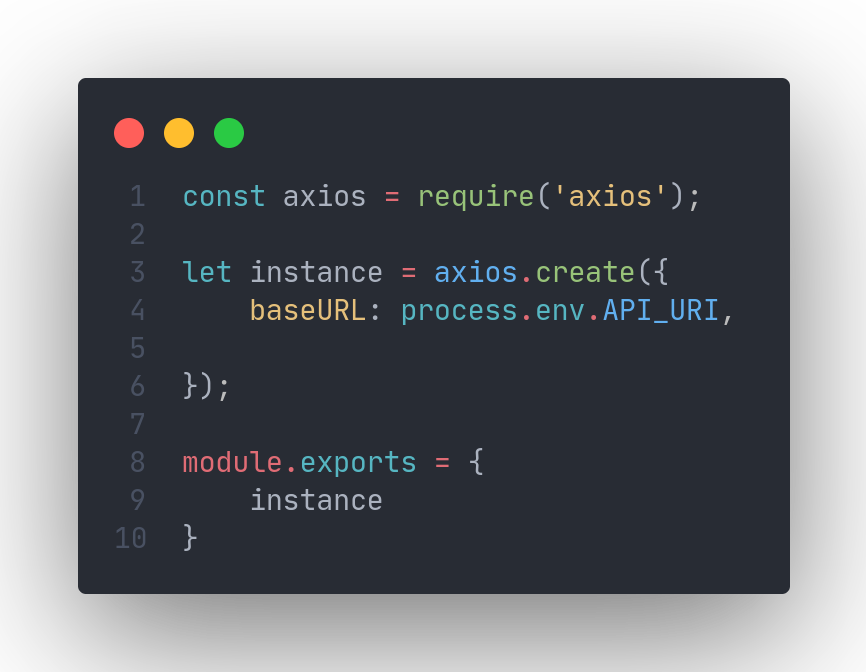
\includegraphics[scale=.4]{assets/images/axios-config.png}
    \caption{Configuracion de Axios}
\end{figure}

Como observamos creamos una nueva instancia de axios con la url del sitio ya cargada en una variable de entorno.

De igual manera se cargo la API KEY en otro variable de entorno, esto para tener un mejor manejo de la seguridad.

\section{Peticion desde axios}

Creamos un archivo que nos sirve ce controlador, aqui definimos un método que nos permitirá obtner los datos de la API. Utilizamos la instancia de axios creada anteriormente

\begin{figure}[H]
    \centering
    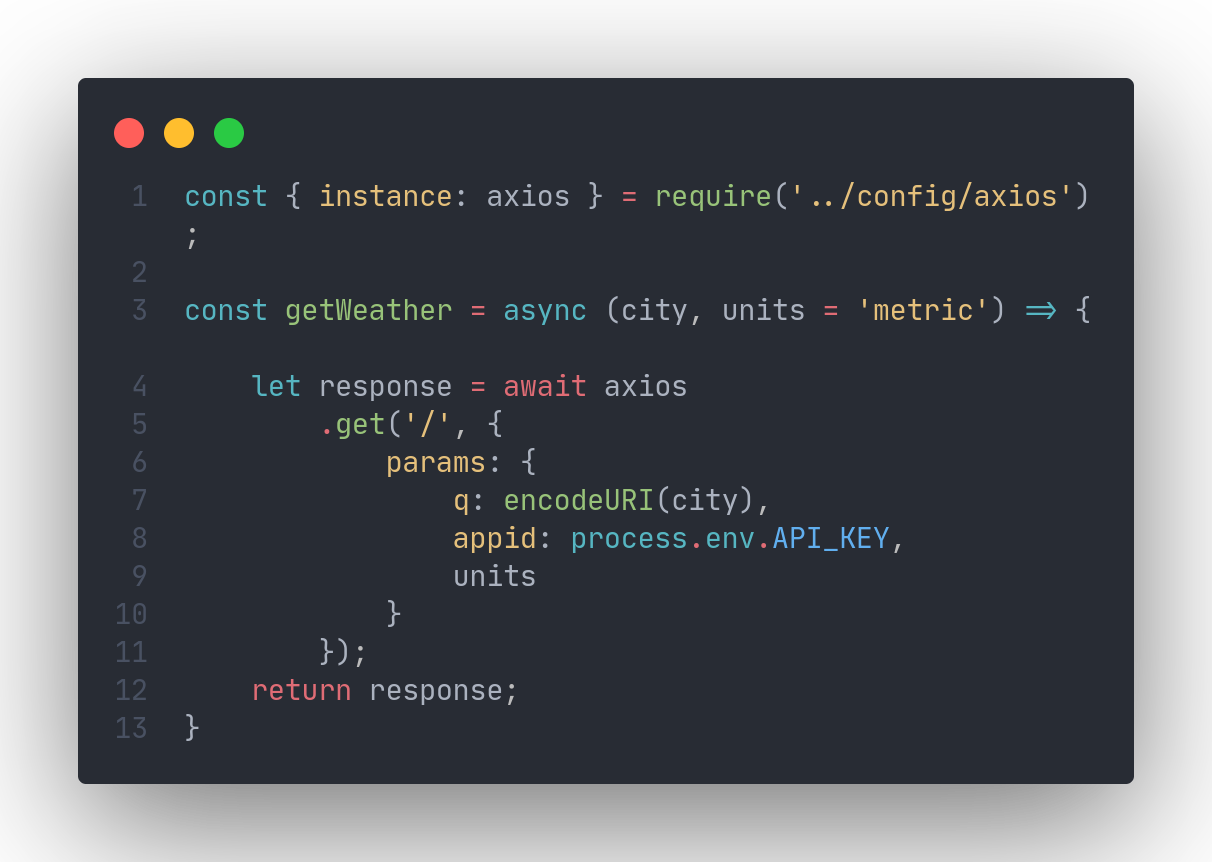
\includegraphics[scale=.3]{assets/images/axios-request.png}
    \caption{Peticion desde axios}
\end{figure}

Como esta instancia de axios esta configurada ya con la url basta con realizar la peticion a la raiz, ademas de enviar los parametros necesarios que son la ciudad y la api key, ademas de las unidades para que obtenga la temperatura en grados celcious.

\section{App}

Ahora solo nos hace falta llamar el método y manejar los datos para que se muestren por pantalla.

\begin{figure}[H]
    \centering
    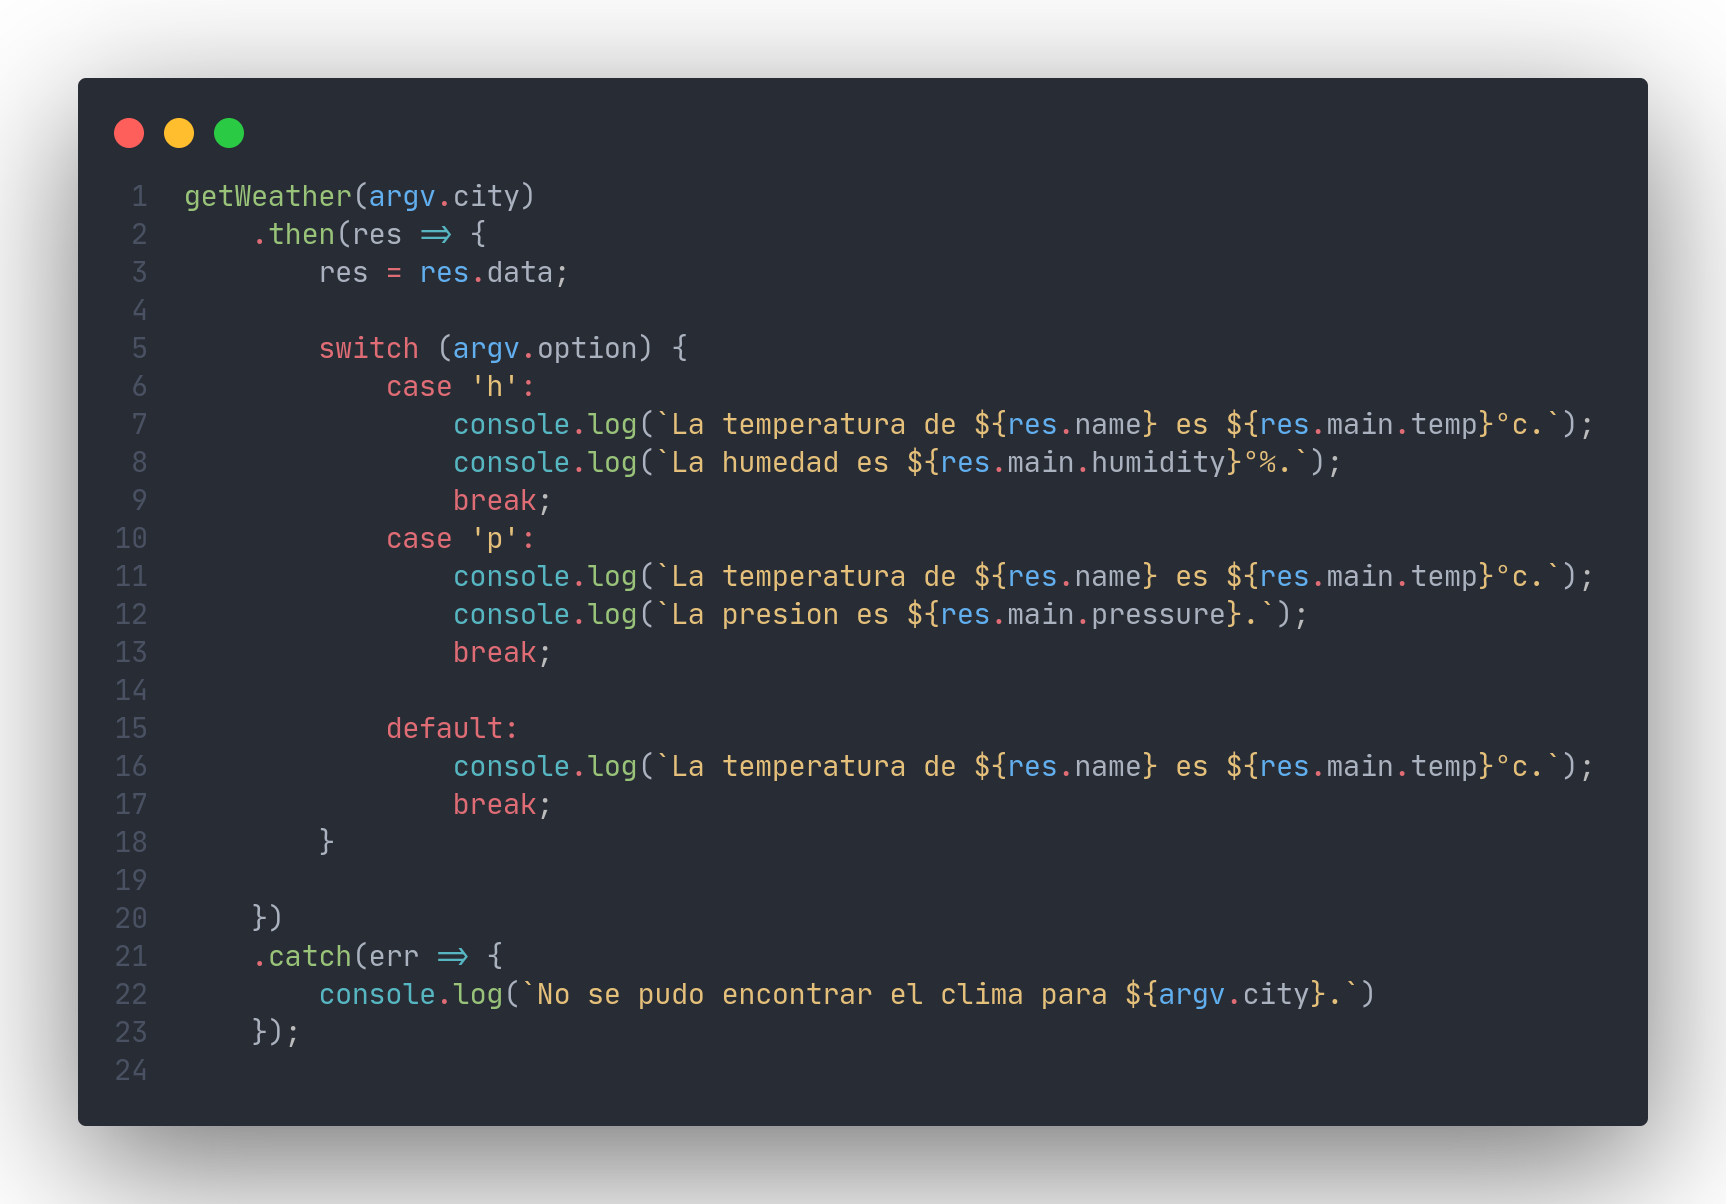
\includegraphics[scale=.22]{assets/images/app.png}
    \caption{Lógica de app.js}
\end{figure}

Una vez ejecutamos el programa obtenemos los siguientes resultados:

\begin{figure}[H]
    \centering
    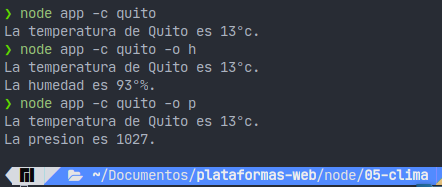
\includegraphics[scale=.75]{assets/images/app-1.png}
    \caption{Ejemplo de ejecucion}
\end{figure}


\end{document}